\subsection{Rancangan Penegakan Otoritas}
\label{subsec:rancangan-penegakan-otoritas}

% Rancangan penegakan otoritas pada subbab ini direferensikan sebagai \texttt{R-TA-05} untuk verifikasi \textit{caveats}, \textit{effective capability}, dan bukti kepemilikan \textit{wallet}, \texttt{R-TA-06} untuk validasi subrole tenaga medis terhadap dataset, serta \texttt{R-TA-07} untuk pencabutan akses token Macaroon delegasi. Rancangan ini merealisasikan \texttt{S-TA-04}, \texttt{S-TA-05}, dan \texttt{S-TA-06} untuk menjawab \texttt{M-TA-01}, \texttt{M-TA-02}, \texttt{M-TA-04}, \texttt{M-TA-05}, \texttt{M-TA-06}, dan \texttt{M-TA-07}.

Penegakan otoritas pada rancangan ini merujuk pada proses memastikan \textit{request} akses terhadap data RME hanya dilayani apabila aktor yang mengajukan permintaan memiliki kewenangan yang sah.

Bagian ini membahas tiga aspek utama penegakan otoritas pada \textit{Server} PRE. Pertama, Subbab \ref{subsubsec:verifikasi-caveats-macaroons-di-pre} menjelaskan verifikasi \textit{caveats} Macaroon untuk memastikan token masih valid. Kedua, Subbab \ref{subsubsec:verifikasi-role-tenaga-medis-untuk-akses-dataset} membahas validasi tambahan terhadap \textit{subrole} \texttt{MedicalPersonnel} agar akses tulis hanya dapat dilakukan pada \textit{dataset category} yang sesuai dengan kewenangannya. Ketiga, Subbab \ref{subsubsec:pencabutan-hak-akses-macaroon-delegasi} menjelaskan rancangan mekanisme revokasi token Macaroon, termasuk revokasi agar token turunannya tidak dapat digunakan.

Sebagai gambaran, Gambar \ref{fig:seqdiag-overview-penegakan-otoritas} menunjukkan alur penegakan otoritas pada \textit{Server} PRE. Secara garis besar, alur akses dimulai dengan aktor melalui \textit{client} untuk mengirimkan permintaan akses ke \textit{Server} PRE. \textit{Server} PRE kemudian memverifikasi token Macaroon, memverifikasi status revokasi dari token, dan menentukan aktor aktif. Jika semua verifikasi berhasil, \textit{Server} PRE melanjutkan proses ke 3 kemungkinan skenario, yaitu mengambil daftar RME yang dapat diakses, melakukan pembacaan data RME yang melibatkan proses \textit{re-encryption}, dan melakukan penulisan data RME.

\begin{figure}[!ht]
	\centering
	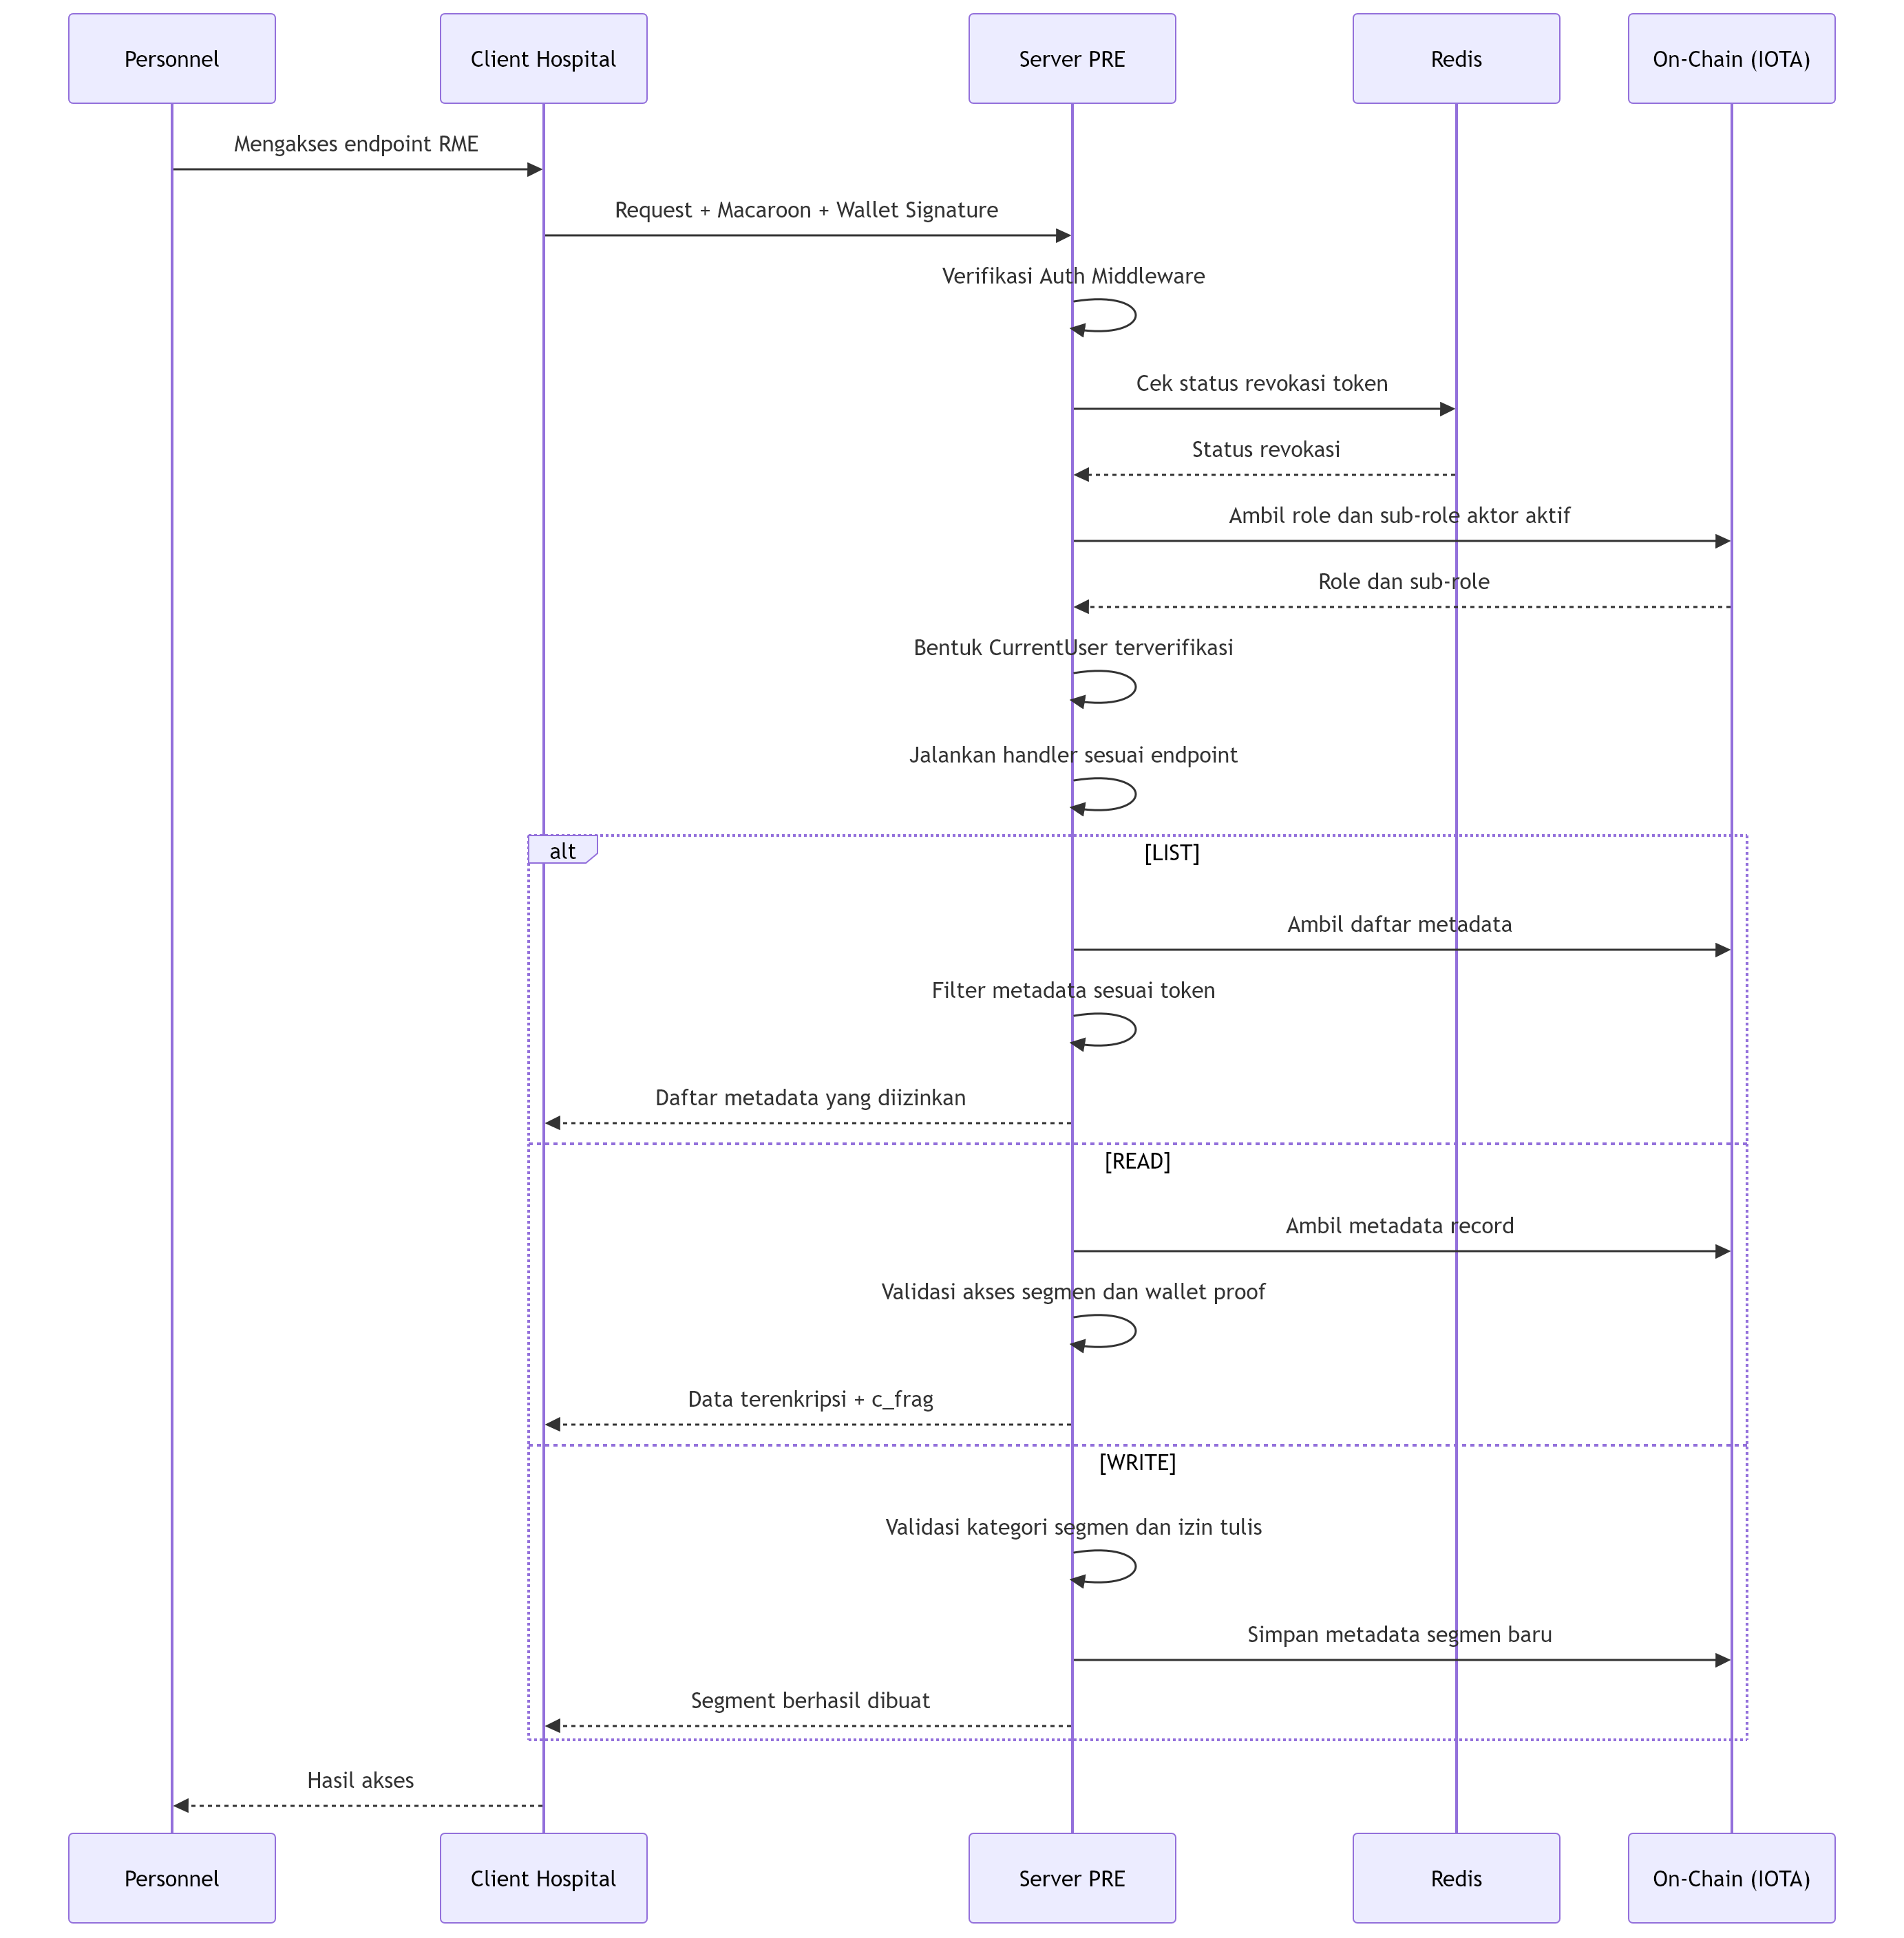
\includegraphics[width=\textwidth]{resources/chapter-3/rancangan/penegakan otoritas/seqdiag-overview.png}
	\caption{Alur penegakan otoritas pada \textit{Server} PRE}
	\label{fig:seqdiag-overview-penegakan-otoritas}
\end{figure}

\subsubsection{Verifikasi \textit{Caveats} Macaroons}
\label{subsubsec:verifikasi-caveats-macaroons-di-pre}

\textit{Server} PRE bertindak sebagai titik penegakan kebijakan akses. \textit{Server} PRE memverifikasi token Macaroon dan seluruh \textit{caveats}. Jika terdapat \textit{caveat} yang tidak dikenali atau diluar rancangan pada Tabel \ref{tab:rancangan-caveats-macaroons-baru}, permintaan akses ditolak.

Rancangan langkah verifikasi token Macaroon untuk permintaan akses baca data RME adalah sebagai berikut:

\begin{enumerate}[leftmargin=*]
	\item \textit{Server} PRE memverifikasi validitas token Macaroon melalui mekanisme \textit{Chained-HMAC} menggunakan \texttt{RootKey}.
	\item \textit{Server} PRE memverifikasi bahwa \texttt{patient\_address} dan \texttt{related\_rme\_id} pada token sesuai dengan data RME yang diminta.
	\item \textit{Server} PRE menghitung aktor aktif. Jika tidak terdapat \texttt{delegated\_to}, maka aktor aktif adalah \texttt{root\_subject}. Jika terdapat satu atau lebih \texttt{delegated\_to}, maka aktor aktif adalah nilai \texttt{delegated\_to} terakhir.
	\item \textit{Server} PRE memverifikasi tanda tangan \textit{wallet} dari aktor aktif pada permintaan akses.
	\item \textit{Server} PRE menghitung kedalaman delegasi berdasarkan jumlah \texttt{delegated\_to} pada token dan memastikan nilainya tidak melebihi \texttt{max\_delegation\_depth}.
	\item \textit{Server} PRE memvalidasi seluruh batas waktu pada \texttt{expires\_before} dan menggunakan batas waktu yang paling awal sebagai masa berlaku efektif token.
	\item \textit{Server} PRE menghitung cakupan akses efektif berdasarkan irisan seluruh \texttt{read\_dataset\_in}, \texttt{write\_dataset\_in}, \texttt{read\_function\_in}, dan \texttt{write\_function\_in}.
	\item \textit{Server} PRE mengambil metadata segmen dari IOTA dan mencocokkan \texttt{dataset\_category} serta \texttt{function\_category} segmen dengan cakupan akses efektif token.
	\item Jika seluruh verifikasi berhasil, \textit{Server} PRE melanjutkan proses pengambilan data terenkripsi dari IPFS dan melakukan \textit{re-encryption}. Jika salah satu pemeriksaan gagal, permintaan akses ditolak.
\end{enumerate}

\subsubsection{Verifikasi \textit{Role} dan \textit{Subrole} Tenaga Medis untuk Akses \textit{Dataset}}
\label{subsubsec:verifikasi-role-tenaga-medis-untuk-akses-dataset}

Dari hasil analisis pada Subbab \ref{subsec:analisis-verifikasi-aktor-operasi-tulis}, diperlukan verifikasi tambahan terhadap \textit{subrole} \texttt{MedicalPersonnel} agar akses tulis hanya dapat dilakukan pada \textit{dataset category} yang sesuai dengan kewenangannya. Pada implementasi Tugas Akhir ini, terdapat 4 \textit{subrole} turunan dari \textit{role} \texttt{MedicalPersonnel}, yaitu dokter, perawat, petugas laboratorium, dan apoteker. Sebagaimana dijelaskan pada Subbab \ref{subsec:analisis-segmentasi-data-rme}, setiap \textit{subrole} tersebut memiliki kebutuhan akses data yang berbeda-beda untuk melakukan akses jenis \textit{update}. Pemetaan kebutuhan akses data untuk setiap \textit{subrole} dapat dilihat pada Tabel \ref{tab:pemetaan-hak-akses-update-subrole}.

\begin{table}[!ht]
	\centering
	\caption{Pemetaan Hak Akses Update Berdasarkan subrole Tenaga Medis}
	\label{tab:pemetaan-hak-akses-update-subrole}
	\begin{tabular}{|p{0.15\textwidth}|p{0.35\textwidth}|p{0.35\textwidth}|}
		\hline
		\textbf{\textit{subrole}} & \textbf{\textit{Dataset Category}} & \textbf{\textit{Function Category}}                  \\
		\hline
		Perawat                   & Rawat Jalan/Rawat Inap             & Anamnesis, Pemeriksaan Fisik, Pemeriksaan Psikologis \\
		\hline
		Dokter                    & Rawat Jalan/Rawat Inap             & Seluruh \textit{function category}                   \\
		\hline
		Lab                       & Laboratorium                       & Laboratorium                                         \\
		\hline
		Apoteker                  & Apotek                             & Peresepan dan Dispensing                             \\
		\hline
	\end{tabular}
\end{table}

Berdasarkan pemetaan tersebut, terdapat verifikasi tambahan untuk \textit{role} \texttt{MedicalPersonnel}, yaitu melakukan validasi apakah \textit{subrole} pengguna yang saat ini mencoba melakukan aksi \textit{write} memang sesuai dengan jenis \textit{dataset} yang diakses. Alur tambahan tersebut ditunjukkan pada Gambar \ref{fig:seqdiag-validasi-subrole-dataset}. Pada alur ini, \textit{Server} PRE terlebih dahulu mendapatkan informasi \textit{subrole} tenaga medis melalui \textit{smart contract}. Informasi tersebut kemudian digunakan untuk memvalidasi pasangan \textit{role} dan \textit{subrole} terhadap kategori \textit{dataset} yang coba ditulis. Apabila \textit{subrole} aktor tidak memiliki kewenangan untuk menulis pada kategori \textit{dataset} tersebut, maka \textit{request} ditolak. Bagian berlatar merah pada Gambar \ref{fig:seqdiag-validasi-subrole-dataset} menunjukkan alur yang berubah atau ditambahkan pada rancangan Tugas Akhir ini dibandingkan Implementasi DecMed sebelumnya. Perubahan tersebut mencakup pengambilan informasi \textit{subrole} dari \textit{smart contract} serta validasi kesesuaian \textit{role}, \textit{subrole}, dan kategori \textit{dataset} sebelum akses tulis diberikan.

\begin{figure}[!ht]
	\centering
	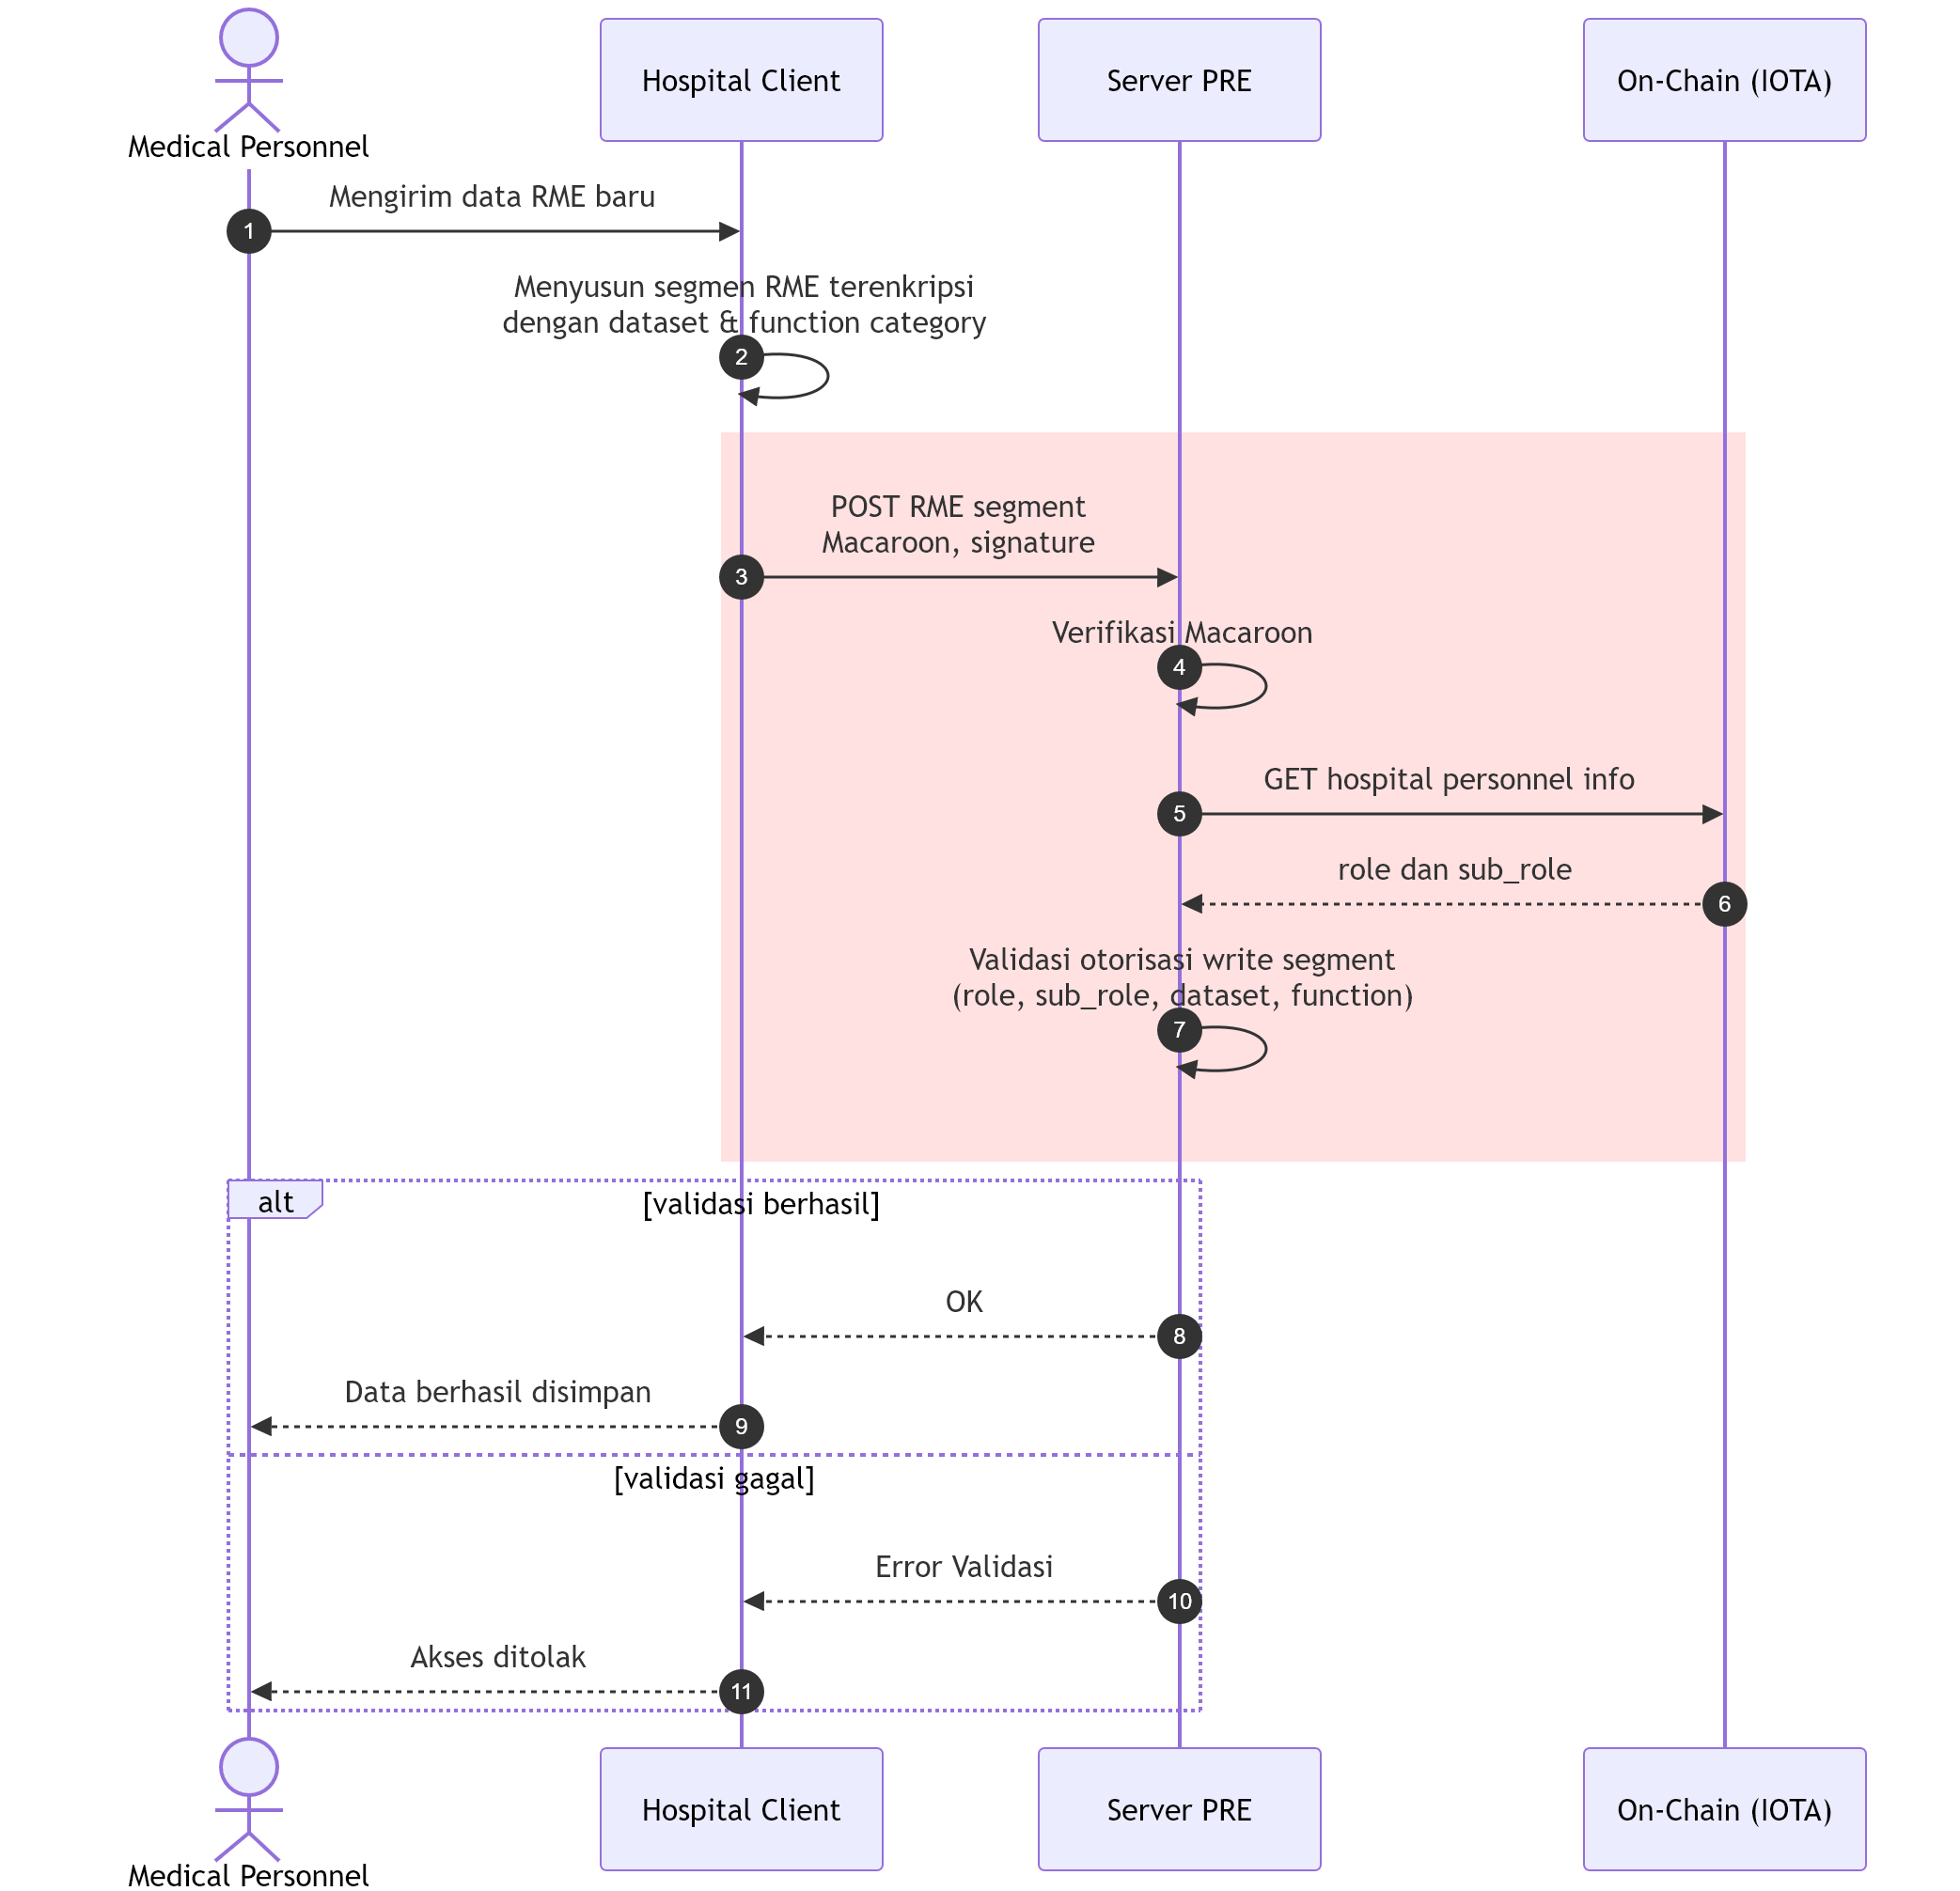
\includegraphics[width=0.95\textwidth,height=0.80\textheight,keepaspectratio]{resources/chapter-3/rancangan/seqdiag-validasi-subrole X dataset.png}
	\caption{\textit{Sequence Diagram} Rancangan Validasi \textit{subrole} Tenaga Medis terhadap \textit{Dataset Category}}
	\label{fig:seqdiag-validasi-subrole-dataset}
\end{figure}

Validasi menggunakan data \textit{role} dan \textit{subrole} yang terdapat pada penyimpanan\textit{on-chain} karena pada Macaroon tidak terdapat informasi \textit{role} dari pengguna aktif saat ini, sesuai dengan rancangan \textit{caveats} pada Tabel \ref{tab:rancangan-caveats-macaroons-baru}. Sementara itu, \textit{registry personnel} pada penyimpanan \textit{on-chain} merepresentasikan status kelembagaan aktor, misalnya apakah aktor masih terdaftar sebagai \textit{personnel} rumah sakit dengan \textit{role} atau \textit{subrole} tertentu. Dengan demikian, \textit{request} hanya dilanjutkan apabila aktor memiliki token yang valid sekaligus masih memiliki otoritas kelembagaan yang sesuai.

\subsubsection{Verifikasi \textit{Wallet} Aktor Aktif}
\label{subsubsec:verifikasi-wallet-aktor-aktif}

Sesuai analisis pada Subbab \ref{subsec:verifikasi-bukti-kepemilikan-wallet}, diperlukan verifikasi tambahan terhadap \textit{wallet} aktor aktif untuk memastikan \textit{request} dilakukan oleh aktor aktif yang sah.

Rancangan proses verifikasi dilakukan dengan mekanisme \textit{presigned request}. Ketika \textit{client} mengirimkan \textit{request} ke \textit{Server} PRE, \textit{client} juga menambahkan header yang berisi konteks \textit{request} yang telah di-\textit{sign} menggunakan kunci privat \textit{wallet} pengguna. Konteks \textit{request} memuat informasi seperti \texttt{token\_id}, \texttt{patient\_address}, \texttt{related\_rme\_id}, \texttt{operation}, \texttt{segment\_id}, \texttt{dataset\_category}, \texttt{function\_category}, dan \texttt{timestamp}. Keberadaan \textit{timestamp} pada konteks yang ditandatangani juga membuat \textit{signature} hanya berlaku untuk rentang waktu tertentu. Apabila \textit{signature} tidak valid maka \textit{request} ditolak.

\subsubsection{Pencabutan Hak Akses Macaroon Delegasi}
\label{subsubsec:pencabutan-hak-akses-macaroon-delegasi}

Sesuai dengan analisis pada Subbab \ref{subsec:analisis-revokasi-audit-delegasi}, diperlukan mekanisme revokasi dan audit delegasi untuk memastikan bahwa pencabutan akses dapat berdampak pada seluruh token turunan yang berasal dari token tersebut. Revokasi akses pada implementasi Tugas Akhir ini masih menjadikan pasien sebagai \textit{resource owner} yang berwenang untuk mencabut akses terhadap RME.

Revokasi akses pada implementasi ini dilakukan melalui kombinasi pencatatan status di IOTA \textit{on-chain} dan Redis PRE, dengan \textit{server} PRE bertindak sebagai titik penegakan kebijakan akses. Lapisan \textit{on-chain} digunakan untuk mencatat perubahan status akses dan audit trail revokasi, sedangkan Redis PRE digunakan untuk menyimpan \textit{hash} dari token yang telah dicabut. Alur pencabutan akses oleh pasien ditunjukkan pada Gambar \ref{fig:seqdiag-revoke-access}. Pada alur tersebut, pasien memilih akses yang akan dicabut melalui \textit{Patient Client}. \textit{Patient Client} kemudian mengeksekusi fungsi \texttt{revoke\_access()} pada \textit{smart contract} Move untuk menandai akses sebagai dicabut, menghapus hak akses pada penyimpanan \textit{on-chain}, melakukan pencabutan berantai terhadap penerima delegasi turunan, serta mencatat kejadian revokasi ke dalam \textit{audit log}. Setelah transaksi \textit{on-chain} berhasil, \textit{Patient Client} mengirimkan \textit{payload} revokasi ke \textit{Server} PRE agar menyimpan \textit{hash} dari token yang telah dicabut pada Redis PRE dan menghapus \textit{re-encryption key} terkait dengan token Macaroon yang direvokasi.

\begin{figure}[!ht]
	\centering
	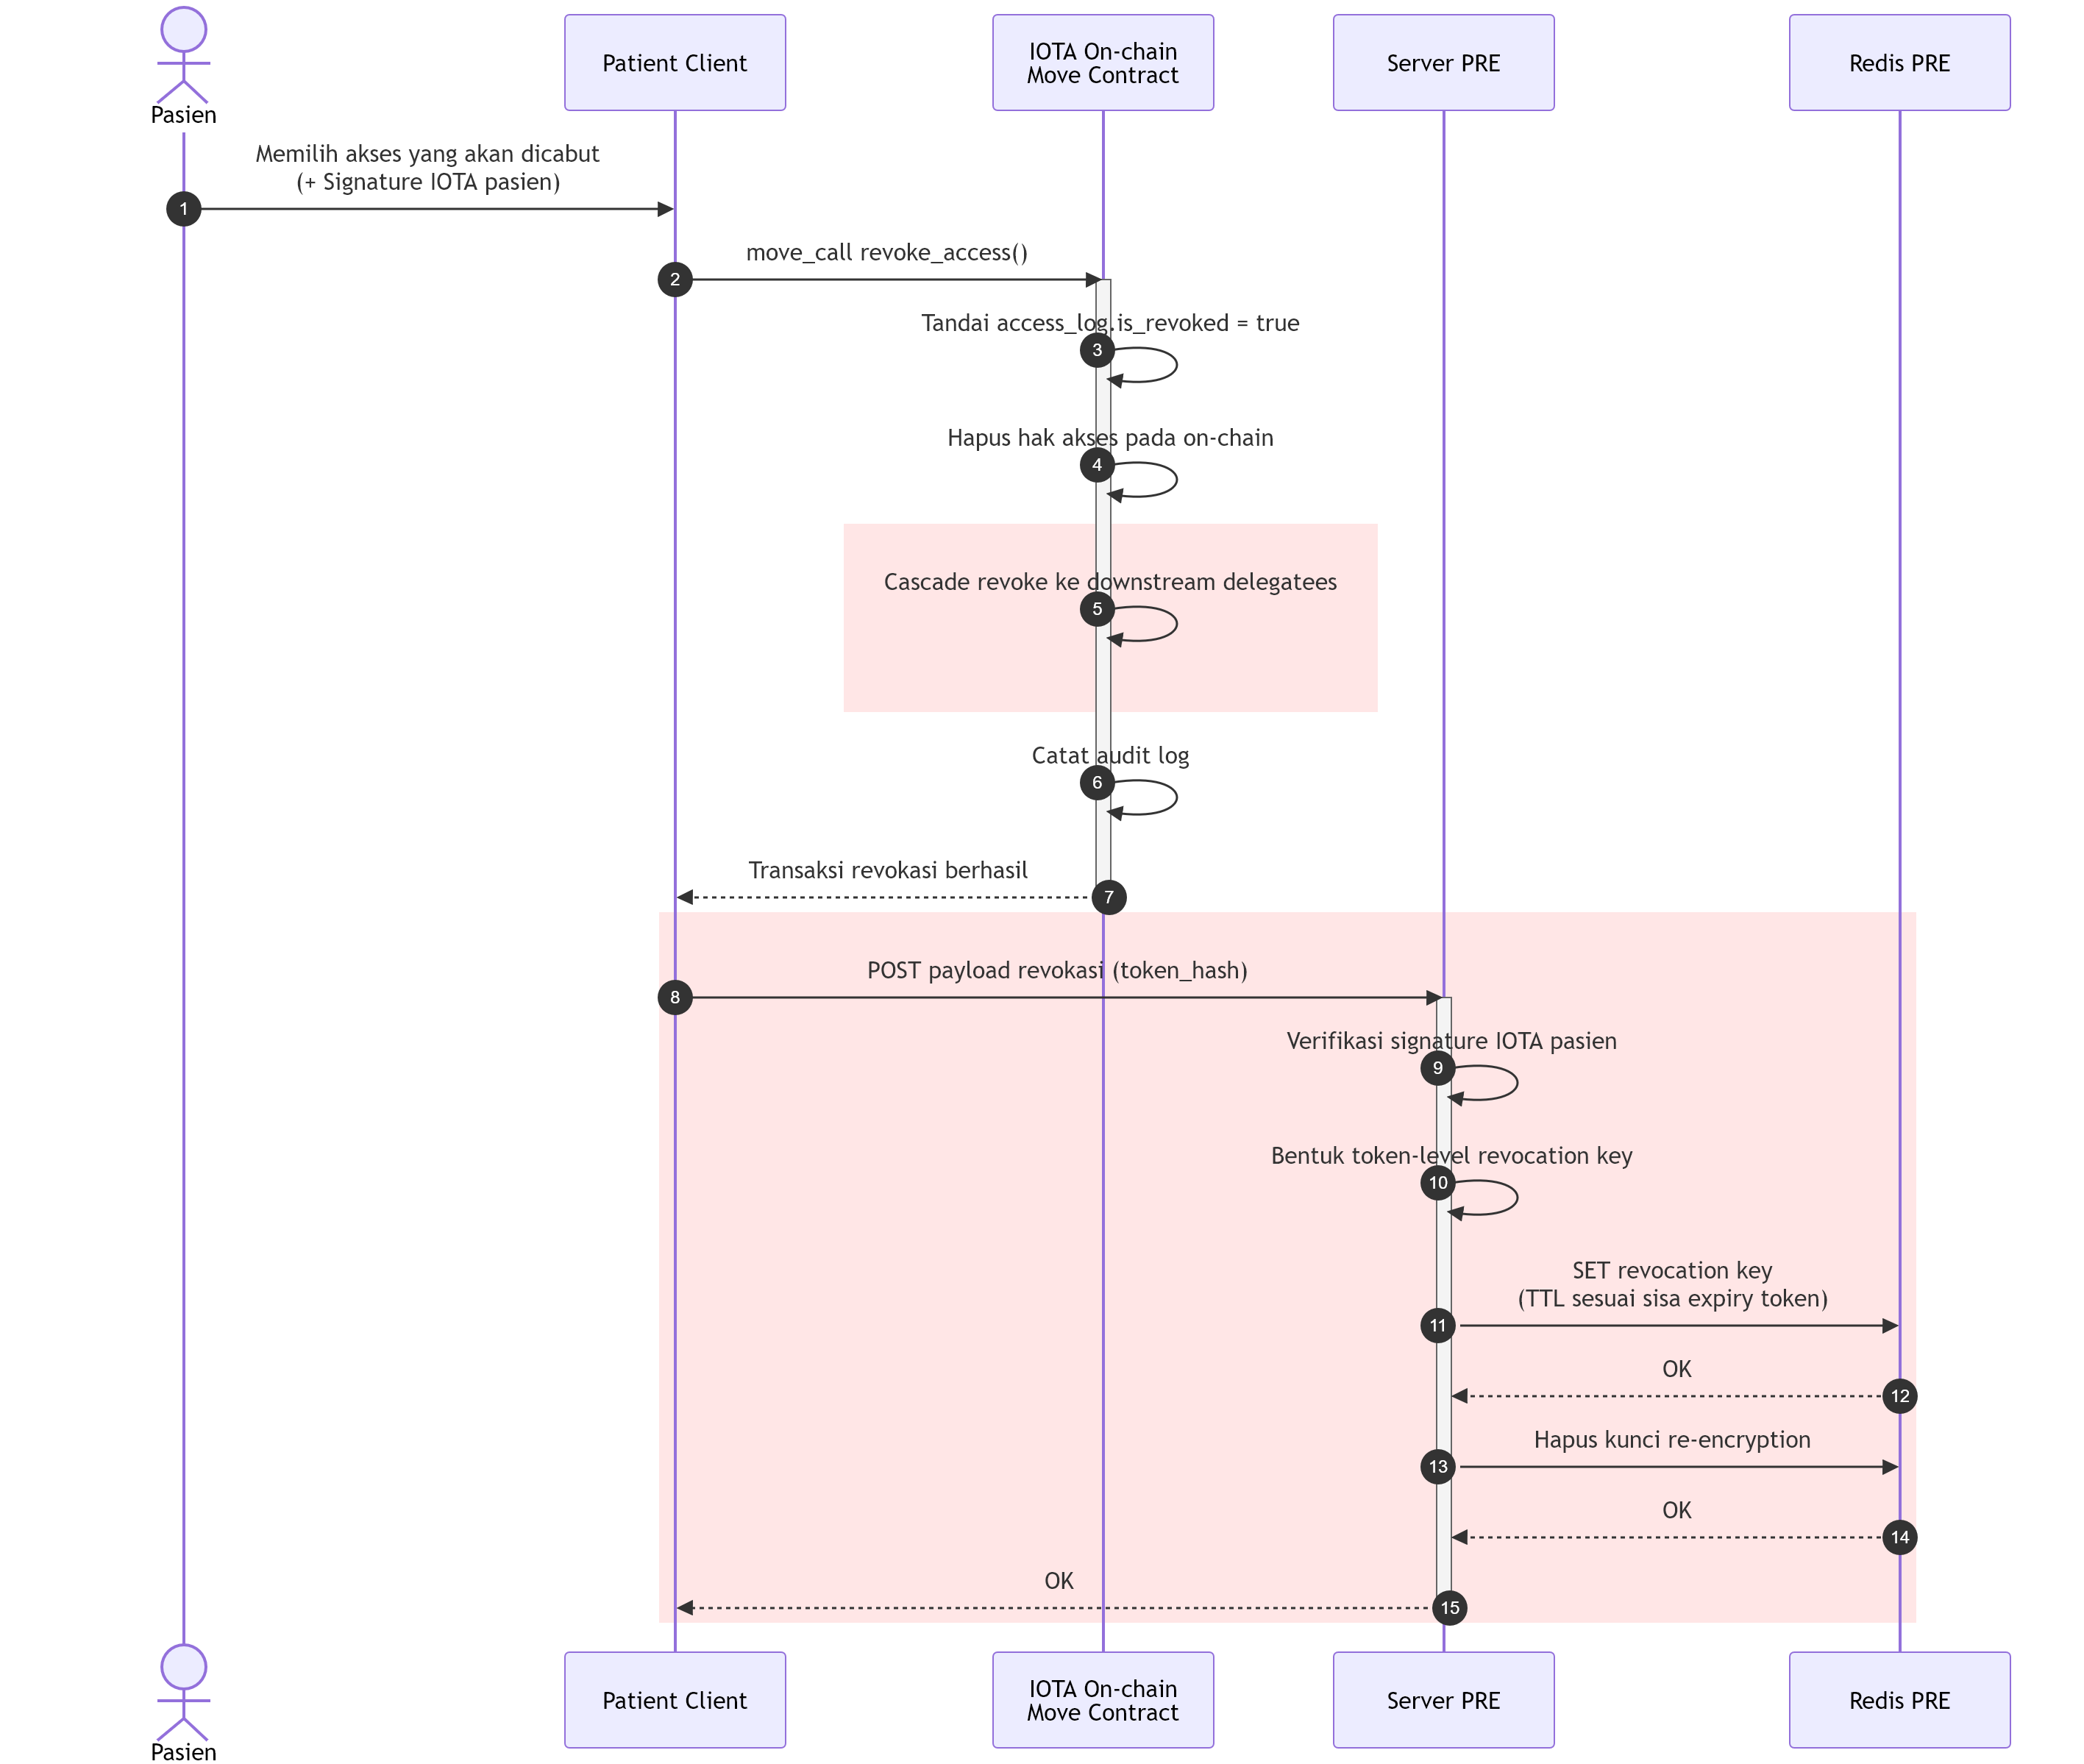
\includegraphics[width=0.95\textwidth,height=0.80\textheight,keepaspectratio]{resources/chapter-3/rancangan/seqdiag-revoke_access.png}
	\caption{\textit{Sequence Diagram} Rancangan Alur Pencabutan Hak Akses Macaroon Delegasi}
	\label{fig:seqdiag-revoke-access}
\end{figure}

Bagian berlatar merah pada Gambar \ref{fig:seqdiag-revoke-access} menunjukkan alur baru yang ditambahkan pada Tugas Akhir ini. Alur baru tersebut mencakup pencabutan berantai terhadap seluruh \textit{downstream delegatees}, pengiriman \textit{payload} revokasi ke \textit{Server} PRE, pembentukan \textit{revocation key}, penyimpanan status revokasi pada Redis dengan TTL sesuai masa berlaku token, serta penghapusan kunci \textit{re-encryption}. Dengan penambahan alur ini, revokasi tidak hanya tercatat pada IOTA, tetapi juga langsung ditegakkan oleh \textit{Server} PRE ketika token Macaroon digunakan kembali.

Pada saat verifikasi, \textit{Server} PRE memeriksa \textit{hash} token yang sedang digunakan dan setiap \textit{caveat} \texttt{parent\_token\_hash} ke \textit{revocation key} pada Redis.  Dengan demikian, apabila pasien mencabut akses pada delegator awal, maka token Macaroon turunan yang dibuat dari akses tersebut juga akan dianggap tidak valid. Selain itu, pemerikskaan status hak akses juga dilakukan pada penyimpanan \textit{on-chain} yang mencatat status hak akses.